\documentclass[10pt,a4paper]{article}
\usepackage{fontspec}
\setmainfont{texgyretermes}[Extension=.otf,UprightFont=*-regular,BoldFont=*-bold,ItalicFont=*-italic,BoldItalicFont=*-bolditalic]
\usepackage[margin=1.8cm,headheight=14pt]{geometry}
\usepackage{amsmath,amssymb,booktabs,tabularx,array,ragged2e,enumitem,microtype,xcolor,tikz,fancyhdr,titlesec,graphicx,caption}
\usetikzlibrary{arrows.meta,positioning,fit,backgrounds}
\usepackage[hidelinks,unicode]{hyperref}
\definecolor{ink}{HTML}{183A45}\definecolor{teal}{HTML}{087F7A}\definecolor{blue}{HTML}{405F8A}\definecolor{gray}{HTML}{56656B}
\newcolumntype{P}[1]{>{\RaggedRight\arraybackslash}p{#1}}
\newcolumntype{Y}{>{\RaggedRight\arraybackslash}X}
\renewcommand{\tabularxcolumn}[1]{>{\RaggedRight\arraybackslash}p{#1}}
\setlength{\parindent}{0pt}\setlength{\parskip}{5pt}\setlength{\emergencystretch}{2em}
\setlength{\tabcolsep}{4pt}\renewcommand{\arraystretch}{1.12}
\setlist{nosep,leftmargin=1.4em,topsep=3pt}
\titleformat{\section}{\large\bfseries\color{ink}}{\thesection}{.6em}{}
\titleformat{\subsection}{\normalsize\bfseries\color{ink}}{\thesubsection}{.6em}{}
\titleformat{\subsubsection}{\normalsize\bfseries}{\thesubsubsection}{.6em}{}
\titlespacing*{\section}{0pt}{8pt}{6pt}\titlespacing*{\subsection}{0pt}{7pt}{4pt}
\pagestyle{fancy}\fancyhf{}
\fancyhead[L]{\small\color{gray}GEOI-BQ: BẢO VỆ QUỸ ĐẠO VÀ ĐÁNH GIÁ ĐỐI CHỨNG}
\fancyhead[R]{\small\color{gray}28/10/2026}\fancyfoot[C]{\small\thepage}
\renewcommand{\headrulewidth}{.3pt}
\renewcommand{\refname}{References}
\renewcommand{\contentsname}{Mục lục}
\setcounter{tocdepth}{3}
\captionsetup{font=small,labelfont=bf}
\newcommand{\key}[1]{\par\smallskip\textcolor{teal}{\textbf{#1}}\par\smallskip}
\newcommand{\claim}[1]{\par\textbf{Ý nghĩa.} #1\par}
\newcommand{\TV}{\operatorname{TV}}
\hypersetup{pdftitle={GeoI-BQ: phương pháp Geo-I và đánh giá đối chiếu paper adaptations},pdfauthor={}}
\newcommand{\PrimaryRecall}{99{,}595}
\newcommand{\PrimaryCI}{[99{,}224; 99{,}903]}
\newcommand{\RatioUpper}{2{,}437372}
\newcommand{\PosteriorUpper}{70{,}91}

\begin{document}
\pagenumbering{roman}
{\setlength{\parskip}{0pt}\tableofcontents}
\clearpage
\pagenumbering{arabic}
\begin{center}
{\LARGE\bfseries\color{ink}Bảo vệ quỹ đạo cho người dùng dịch vụ vị trí}\\[4pt]
{\large Phương pháp dựa trên Geo-I với cận tiết lộ toàn transcript}\\[3pt]
{\small Bản sơ bộ khoa học: đặc tả, chứng minh và đối chiếu thực nghiệm}
\end{center}
\section{Introduction}
\textbf{Motivation.} Dịch vụ dựa trên vị trí (LBS) giúp người dùng tìm địa điểm quan tâm (POI) khi di chuyển.
Những yêu cầu liên tiếp đồng thời tạo thành dấu vết mà nhà cung cấp có thể kết hợp với bản đồ và lịch sử
để suy luận vị trí, đường đi hoặc các thông tin liên quan. Bảo vệ một điểm gửi riêng lẻ vì vậy chưa đủ
để mô tả rủi ro của cả quá trình sử dụng dịch vụ. Các nghiên cứu về bối cảnh giao thông, ngữ nghĩa và
query liên tục đã khai thác những tương quan này\cite{transprotect,semantic,fake}.

\textbf{Các vấn đề cần giải quyết.} Thứ nhất, cơ chế nhiều bước phải tính cả quyết định khi nào cập nhật
thông tin vị trí, không chỉ việc thêm nhiễu. Thứ hai, đầu ra giả có thể hợp lý về hình học nhưng không
lấy được POI phù hợp cho người dùng. Thứ ba, các công trình được khảo sát dùng output, attacker, dữ liệu
và metrics khác nhau: một tọa độ thay thế, một tập chứa GPS thật và các dummy, hoặc một bộ dữ liệu
trajectory được tổng hợp offline không thể được so sánh bằng một score không đổi ý nghĩa.

Vấn đề đánh giá không nằm ở việc hoàn toàn thiếu dataset hoặc metrics trong lĩnh vực. Điều còn thiếu
cho phép đối chiếu ở đây là \emph{một protocol thống nhất giữa những hợp đồng đầu ra và mục tiêu đang xét}.
Luận văn do đó hệ thống hóa các tác vụ suy luận, xây dựng workload có kiểm soát và sử dụng hai lớp đo:
metrics chung theo tác vụ, cùng metrics gốc khi định nghĩa và đầu vào tương thích.

\begin{tabularx}{\linewidth}{@{}P{2.1cm}P{5.6cm}Y@{}}\toprule
\textbf{Nhóm} & \textbf{Mục tiêu} & \textbf{Vai trò nghiên cứu}\\\midrule
S1--S3 & Vị trí hiện tại, nơi dừng, đường đã đi & Tác vụ định vị/tái dựng theo các phạm vi quan sát.\\
S4--S6 & Liên kết người/xe, cạnh kế tiếp, đích tương lai & Suy luận phụ thuộc prior và quan hệ giữa target với trajectory.\\
S7--S8 & Nội dung/ý định query; thông tin người đi cùng & Phân biệt payload với intent, cá nhân với tương quan nhóm.\\
S9--S10 & Điểm đầu và điểm cuối phiên & Rủi ro endpoint dưới mô hình quan sát được khai báo.\\\bottomrule
\end{tabularx}

\textbf{Hướng giải quyết.} GeoI-BQ giữ Geo-indistinguishability (Geo-I) làm nền tảng. Thiết bị dùng REM
và phép thử tái sử dụng có nhiễu để duy trì điểm tham chiếu Z. Từ lịch sử đã bảo vệ, một belief gần đúng
đánh giá những vị trí người dùng có thể ở. Belief điều chỉnh phân phối chọn \emph{đoạn Q} trong giới hạn;
các khung Q được phát theo lịch, còn GPS hiện tại và nhu cầu thật chỉ dùng tại bộ lọc/xếp hạng local.
Phân tích toán học nối các thao tác này thành cận cho toàn transcript trước khi đọc benchmark.

\textbf{Đóng góp chính.}
\begin{enumerate}
\item Hệ thống hóa bài toán thành các scenario, ranh giới quan sát và protocol đánh giá theo output contract;
xây dựng workload SUMO/POI để đo suy luận vị trí, chất lượng đáp án và chi phí trên cùng dữ liệu.
\item Đặc tả phương pháp dựa trên Geo-I và cơ chế chọn chung đoạn Q; phân tích privacy toàn transcript,
giới hạn suy luận và các bảo đảm utility có điều kiện. Không gọi các nền tảng hợp thành/hậu xử lý là định lý mới.
\item Đối chiếu GeoI-BQ với ba adaptation từ nghiên cứu gần đây trên cùng cohort, kèm Raw và REM-Z controls;
giữ CI, failure, metrics không áp dụng và sự khác biệt về chi phí/bảo đảm.
\end{enumerate}
Các kết quả không mặc định bảo vệ đầy đủ S1--S10. Bằng chứng thực nghiệm chính là S1--S3 và S9--S10;
S4--S6 nhận phân tích suy luận có điều kiện, S7 có tính bất biến payload và S8 là hướng mở rộng.

Phần 2 khảo sát nghiên cứu liên quan; Phần 3 trình bày hệ thống, thuật toán và chứng minh; Phần 4 định nghĩa
đánh giá và phân tích thực nghiệm; Phần 5 tổng kết đóng góp, giới hạn và hướng tiếp theo.

\clearpage
\section{Related Work}
\subsection{Truy vấn liên tục và tính hợp lý của đầu ra}
TransProtect\cite{transprotect} khai thác dự đoán chuyển động và chi phí tới đích để chọn miền obfuscation,
đối phó tấn công biết bối cảnh đường/giao thông. Semantic correlation\cite{semantic} xét sự nhất quán
ngữ nghĩa và thời gian của chuỗi tập vị trí. Fake queries\cite{fake} chèn thêm tập toàn giả giữa các lần
truy vấn để làm gián đoạn tương quan và reachability. Những hướng này chỉ ra vì sao attacker không nên
bị giới hạn vào một điểm độc lập; chúng khác nhau ở việc có công bố GPS thật như một thành viên hay không.

\subsection{Geo-I, utility và các phạm vi bảo vệ khác}
EV querying\cite{ev} kết hợp approximate Geo-I với dummy và xử lý cục bộ để giữ chất lượng tìm trạm sạc;
điều đó cho thấy Geo-I + dummy + local selection đã có tiền lệ. PTPPM\cite{ptppm} là preprint road-aware
kết hợp personalized budget và distortion privacy. Khác biệt cần phân tích của GeoI-BQ nằm ở đặc tả
kênh Q và cận toàn transcript, không ở phát biểu rằng lần đầu dùng nhiễu trên mạng đường.

CPCROK\cite{cpcrok} bảo vệ việc nối lại beacon qua pseudonym trong VANET; DP-FETC\cite{dpfetc} phát hành
dataset tổng hợp và xử lý OD/tương quan. Các mục tiêu đó liên quan identity/endpoint nhưng không tự
tương đương tác vụ POI online. SoK\cite{sok} giúp phân biệt đơn vị privacy và các mục tiêu của generative
trajectory publication; nó là nguồn bối cảnh, không là một model đối chứng online.

\subsection{Tổng hợp phạm vi, metrics và khả năng đối chiếu}
Khảo sát phương pháp gần đây dùng cửa sổ \textbf{28/10/2023--28/10/2026}, xét công bố đầu tiên có bằng chứng.
Geo-I 2013 và predictive mechanism 2014 được dẫn riêng ở Phần 3 như nguồn nền tảng.
Trong bảng: \textbf{F} = trực tiếp xét/đánh giá task theo giả định paper; \textbf{P} = một phần hoặc bối cảnh khác;
\textbf{CX} = chưa đủ căn cứ đối chiếu chi tiết. Các nhãn do ta ánh xạ sang S1--S10, không có nghĩa chống mọi attacker.
Scenario không liệt kê chưa có căn cứ coverage trong audit này; không tự quy thành score 0 hoặc đã bảo vệ.

\begin{footnotesize}\par\smallskip\noindent\begin{tabularx}{\linewidth}{@{}P{2.75cm}P{2.15cm}P{1.6cm}P{2.4cm}P{2.5cm}Y@{}}\toprule
\textbf{Paper / cơ chế} & \textbf{Output} & \textbf{Scenario} & \textbf{Privacy} & \textbf{Utility / cost} & \textbf{Tái lập trong bản này} \\
\midrule
\textbf{TransProtect} 2024\cite{transprotect}\newline Học chuyển động + chọn miền + obfuscation & Một tọa độ thay thế/mốc & F: S1, S3\newline P: S2 & EIE; tấn công VehiTrack & Travel-cost distortion $\Delta$c; chi phí vận hành chưa có contract chung & Chạy Markov adaptation; không có checkpoint Transformer gốc \\
\textbf{Semantic correlation} 2026\cite{semantic}\newline Tương quan ngữ nghĩa và thời gian & GPS thật + K-1 dummy & F: S1\newline P: S2, S3 & Anonymity success rate (ASR) & DER là chất lượng dummy; thời gian sinh & Chạy OSM/empirical adaptation; không tái lập AMap/LSTM \\
\textbf{Fake queries} 2026\cite{fake}\newline Chèn query toàn giả giữa query thật & Real+dummy sets và fake packets & F: S1, S3\newline P: S2 & ASR; số đường khó phân biệt & Thời gian/RSS; chưa đo Recall POI chung & Chạy road/history adaptation, giữ fake timing và mọi chi phí \\
\textbf{EV querying} 2024\cite{ev}\newline Approximate Geo-I + dummy + Edge & Vị trí nhiễu và dummy; chọn trạm sạc local & P: S1, S2, S3 & ($\varepsilon$,$\delta$)-AGeoI; IBU/Wasserstein & Cost of Privacy (CoP), tỷ lệ CoP=0 & Khảo sát; chưa có adaptation cùng dịch vụ và giả định Edge \\
\textbf{CPCROK} 2025\cite{cpcrok}\newline Mix-zone, đổi pseudonym và beacon giả & Beacon thật + tuyến beacon giả & P: S4 & Tỷ lệ khớp lại quỹ đạo $\rho$ & Số tuyến giả $\psi$; truyền thông VANET & Khác hợp đồng POI online; không đưa vào bảng score chính \\
\textbf{DP-FETC} 2025\cite{dpfetc}\newline Thống kê DP, tổng hợp trace và chỉnh OD & Bộ dữ liệu quỹ đạo offline & P: S3, S8, S9, S10 & $\varepsilon$-DP; mutual information & JSD phân bố; độ phức tạp & Offline publishing; không chấm bằng request POI online \\
\textbf{PTPPM} 2025\cite{ptppm}\newline Personalized budget, PLS, Permute-and-Flip & Vị trí đã perturb trên mạng đường & CX: S1, S3 & Geo-I + distortion privacy/EIE bound & Perturbation distance/QoS & Preprint liên quan; chưa có comparator đã audit trong repo \\
\textbf{SoK trajectory generation} 2024\cite{sok}\newline Systematization và unit of privacy & Khảo sát phát hành dữ liệu tổng hợp & Không áp dụng & Formal privacy, reconstruction/correlation threats & Mục tiêu và utility của dữ liệu tổng hợp & Nguồn bối cảnh; không là một model đối chứng online \\
\bottomrule\end{tabularx}\par\smallskip
\end{footnotesize}

\textbf{Khoảng trống đánh giá.} ASR đòi một thành viên thật và posterior tương ứng; Q-only không có thành viên
đó. DER đo chất lượng dummy, JSD đo fidelity của dataset và CoP đo tổn thất dịch vụ, không phải cùng một
đại lượng privacy. Vì vậy, Phần 4 định nghĩa metrics chung theo threat và utility thực nhận, đồng thời giữ
metrics gốc đúng contract. Khác định nghĩa phải ghi rõ; thiếu đầu vào giữ N/A, không chuyển thành score tốt.

Ba hàng TransProtect*, Semantic* và Fake-query* trong thực nghiệm là các adaptation đã audit. Những hàng
khác định vị nghiên cứu và giới hạn coverage; chưa có implementation phù hợp thì không được gán số benchmark.

\clearpage
\section{Proposed Method}
\subsection{Problem formulation and assumptions}
Đầu vào riêng là trajectory $X=(x_0,x_1,\ldots)$ tại cùng lịch \emph{có thể đọc}, cùng nhu cầu $\psi_t$.
Bối cảnh $C$ gồm bản đồ, cấu hình, clock và provider law. Lịch sử $E$ chứa các nhánh noisy test và các Z;
$b_t$ là belief gần đúng từ thông tin đã bảo vệ. Đầu ra công khai $O$ gồm các Q có thứ tự, timestamp,
request/reply và retry logic. Đáp án đã lọc ở thiết bị không thuộc $O$.

Một phiên có cùng token/ledger; restart tiếp tục phiên, không cấp lại ngân sách. Attacker là server hoặc
bên có cùng quyền quan sát, biết thuật toán và cấu hình công khai, có thể nối cả transcript. Không giả định
attacker phải biết sẵn hai trajectory thật: hai traces chỉ là phép so sánh trong định lý.

Các kết quả dựa trên: (i) support và xác suất nền chung tại cùng lịch sử phân tích (Q/đoạn, lane giả, replies),
không lọc theo GPS/Z/belief; (ii) downstream chỉ đọc
thông tin đã bảo vệ; (iii) bit đều mới cho kernel Q và ledger không rollback; (iv) cùng clock/provider law;
(v) metadata POI còn hợp lệ cho chứng minh cache. Nhánh Geo-I còn cần sampler lý tưởng và phục hồi đầy đủ
upstream. Hai traces được cố định trước phép chạy; tuyến thật thay đổi do đề xuất POI cần mô hình tương tác riêng.
Account/IP/biển số và kênh thời gian/lỗi ngoài giao thức không được che bởi các định lý này.

\subsection{System architecture}
\begin{center}
\begin{tikzpicture}[>=Latex,b/.style={draw=ink!65,rounded corners=2pt,fill=white,text width=3.2cm,align=center,inner sep=7pt,font=\small},a/.style={->,thick,draw=ink},private/.style={->,thick,draw=teal}]
\node[b] (user) at (0,0) {\textbf{Người dùng / cảm biến}\\GPS $x_t$, nhu cầu $\psi_t$};
\node[b,draw=teal,fill=teal!5] (model) at (5.4,0) {\textbf{GeoI-BQ}\\Bảo vệ / lập kế hoạch Q};
\node[b] (server) at (10.8,0) {\textbf{LBS server}\\Nhận Q; trả POI};
\node[b] (context) at (5.4,-2.3) {\textbf{Ngữ cảnh công khai}\\Bản đồ, cấu hình, POI};
\node[b] (local) at (5.4,-4.8) {\textbf{Xử lý đáp án local}\\Union/cache, lọc, sắp xếp};
\node[b] (out) at (0,-4.8) {\textbf{Đáp án người dùng}\\Danh sách phù hợp\\đã sắp xếp};
\node[b] (attacker) at (10.8,-3) {\textbf{Attacker tại server}\\Lưu Q, clock, replies\\Suy luận trajectory};
\draw[a] (user)--node[above,text width=1.6cm,align=center,font=\scriptsize] {GPS cho lớp\\bảo vệ}(model);
\draw[a] (context)--(model);\draw[a] (model)--node[above,text width=1.6cm,align=center,font=\scriptsize] {Q, request\\chung}(server);
\draw[a] (server.south west)--(8.3,-1.5)--(8.3,-4.8)--node[above,font=\scriptsize] {POI}(local.east);
\draw[a] (local)--(out);\draw[a,dashed] (server)--(attacker);
\draw[private] (user.west)--(-2.2,0)--(-2.2,-3.5)--(5.4,-3.5)--node[right,font=\scriptsize] {GPS + $\psi$ local}(local.north);
\begin{scope}[on background layer]\node[fit=(user)(model)(context)(local)(out),draw=teal,fill=teal!2,rounded corners,inner sep=12pt] {};\end{scope}
\node[font=\small\bfseries,text=teal,fill=white,inner sep=2pt] at (2.7,1.05) {THIẾT BỊ TIN CẬY};
\end{tikzpicture}
\captionof{figure}{Vị trí mô hình trong hệ thống. Chỉ Q/request chung đi sang LBS; GPS và nhu cầu thật phục vụ xếp hạng tại client.}
\label{fig:system}
\end{center}
Server cung cấp dữ liệu; chất lượng sử dụng được đánh giá sau khi client xử lý theo nhu cầu thật. Cache
không tự tạo POI chưa nhận. Năm query slots không đồng nghĩa k-anonymity và Z nội bộ không mặc định là một Q gửi đi.

\clearpage
\subsection{Model architecture and workflow}
\begin{center}
\begin{tikzpicture}[>=Latex,b/.style={draw=ink!65,rounded corners=2pt,fill=white,text width=8cm,align=center,inner sep=6pt,font=\small},e/.style={draw=blue!60,fill=blue!4,rounded corners,text width=3.1cm,align=center,inner sep=5pt,font=\small},a/.style={->,thick,draw=ink}]
\node[e,text width=7.8cm] (gps) at (0,.4) {\textbf{Input: GPS $x_t$ tại mốc được phép đọc}};
\node[b] (rem) at (0,-1) {\textbf{1. REM + noisy reuse + cap Geo-I}\\Tạo Z trên đường hoặc giữ Z cũ; dự toán chi phí trước GPS};
\node[b] (belief) at (0,-2.5) {\textbf{2. Belief từ protected history}\\Dự đoán di chuyển; cập nhật bằng likelihood của Z};
\node[b,draw=teal] (select) at (0,-4) {\textbf{3. Chọn chung một đoạn Q}\\Chấm điểm bằng belief; centered kernel bị chặn\\Thư viện/xác suất nền chỉ dùng thông tin công khai};
\node[b] (send) at (0,-5.6) {\textbf{4. Phát ba khung đã commit}\\0/20/40 s, mỗi khung K5; L60 mỗi loại/Q};
\node[b] (local) at (0,-7.1) {\textbf{5. Union/cache và local ranking}\\GPS hiện tại + nhu cầu thật $\psi_t$};
\node[e,text width=7.8cm] (answer) at (0,-8.5) {\textbf{Output: toàn danh sách phù hợp đã sắp xếp}};
\node[e] (pub) at (6.4,-2.5) {\textbf{Public context}\\Đường, clock, Q trước, replies/cache};
\node[e] (ledger) at (6.4,-4) {\textbf{Ledger Q}\\$\Gamma_Q$, counter, đoạn đã commit};
\node[e] (lbs) at (6.4,-5.6) {\textbf{LBS server}\\Q $\rightarrow$ POI};
\draw[a] (gps)--(rem);\draw[a] (rem)--(belief);\draw[a] (belief)--(select);\draw[a] (select)--(send);\draw[a] (send)--(local);\draw[a] (local)--(answer);
\draw[a,dashed] (pub.west)--(4.5,-2.5)--(4.5,-4)--(select.east);\draw[a,dashed] (ledger.west)--(select.east);
\draw[a,blue] (send.east)--(lbs.west);\draw[a,blue] (lbs.south)--(6.4,-6.5)--(local.east);
\draw[a,teal] (gps.west)--(-5.35,.4)--(-5.35,-7.1)--(local.west);
\node[rotate=90,font=\scriptsize,text=teal] at (-5.55,-3.6) {GPS hiện tại cho local ranking};
\draw[a,dashed] (local.west)--(-4.65,-7.1)--(-4.65,-4)--(select.west);
\begin{scope}[on background layer]\node[fit=(rem)(belief)(select)(send)(local),draw=teal,fill=teal!2,rounded corners,inner sep=10pt] {};\end{scope}
\node[anchor=south west,font=\scriptsize\bfseries,text=teal,fill=white] at (-4.3,-.36) {MÔ HÌNH GEOI-BQ TẠI CLIENT};
\end{tikzpicture}
\captionof{figure}{Kiến trúc nội bộ. Đoạn là đầu ra lấy mẫu chung; từng khung được phát sau đó là hậu xử lý, không chọn lại theo belief giữa đoạn. Mũi tên nét đứt từ local chỉ chuyển cache suy từ replies.}
\label{fig:model}
\end{center}

\begin{tabularx}{\linewidth}{@{}P{3cm}Y@{}}\toprule
\textbf{Thành phần} & \textbf{Cấu hình cuối và lý do}\\\midrule
Geo-I/REM & $B=0{,}24$ m$^{-1}$, $H=12$, $u=B/(2H)=0{,}01$ m$^{-1}$; $M=23$, $C_s=Mu=0{,}23$ m$^{-1}$ mỗi phiên.\\
Noisy test / cadence & Ngưỡng 200 m; private reads cách ít nhất 60 s, nếu đủ dự toán. Gửi Q mỗi 20 s.\\
Q và dịch vụ & K5, ba khung/đoạn; L60 mỗi loại và tọa độ; giữ request chung cho bốn purposes local.\\
Kernel / ledger & $\Gamma_Q=1$, $\varepsilon_{Q,j}=\Gamma_Q/[j(j+1)]$; score integer $S=65536$; commit trước gửi.\\
Public planning & Portfolio beam24; novelty và long-range weight4; travel scale60 s; hold khả thi.\\\bottomrule
\end{tabularx}
Cap bảo vệ tổng tiết lộ; nó không đặt thời gian tối đa được di chuyển. Hết cap thì dùng thông tin đã bảo vệ,
đổi lại khả năng thích nghi giảm. $\Gamma_Q$ không có đơn vị, không cộng trực tiếp với $C_s$ theo m$^{-1}$.

\clearpage
\subsection{Algorithm specification}
\textbf{REM và noisy reuse.} Với miền ứng viên đường công khai $V$ và tọa độ $a_v$:
\begin{equation}
R_u(v\mid x)=\frac{\exp[-u\|x-a_v\|/2]}{\sum_{w\in V}\exp[-u\|x-a_w\|/2]},\quad V_t\sim R_u(\cdot\mid x_t),\quad Z_t=a_{V_t}.
\label{eq:rem}
\end{equation}
Sau lần đầu, ở mốc được phép đọc, đặt $D_t=\mathbf1\{\|x_t-Z_{\rm cũ}\|+\xi_t>200\}$ với
$\xi_t\sim\operatorname{Lap}(0,1/u)$. $D_t=0$ giữ Z; $D_t=1$ tạo Z mới bằng REM. Không có bước planar noise rồi ``map vào REM''.

\textbf{Belief.} Trên các trạng thái đại diện $s$, dự đoán rồi cập nhật:
\begin{equation}
b_t^-(s)=\sum_rb_{t-1}(r)T_{\Delta t}(r,s),\qquad
b_t(s)=\frac{b_t^-(s)\ell_t(Z_t\mid s,Z_{\rm cũ})}{\sum_rb_t^-(r)\ell_t(Z_t\mid r,Z_{\rm cũ})}.
\label{eq:belief}
\end{equation}
Likelihood cộng xác suất các lane trùng tọa độ và tính noisy reuse. Mốc không đọc mới chỉ dự đoán; không coi
Z cũ là một quan sát REM độc lập mới. Lưới, prior và chuyển tiếp là xấp xỉ, không phải posterior đã hiệu chuẩn.

\textbf{Từ belief đến phân phối chọn đoạn.} Mỗi $A_a$ gồm ba khung năm Q khả thi trên đường. Thư viện
và $w_a>0$, $\sum_aw_a=1$ chỉ phụ thuộc public context/history. Belief không loại ứng viên:
\begin{equation}
v_a=\sum_sb(s)g_a(s),\quad z_a=\operatorname{Quantize}(v)_a/S\in[0,1],\quad
\mu=\sum_aw_az_a,\quad \alpha=\frac{\varepsilon_Q}{2+\varepsilon_Q},\quad p_a=w_a[1+\alpha(z_a-\mu)].
\label{eq:kernel}
\end{equation}
$g_a$ là proxy utility công khai; min--max trước lượng tử hóa giữ điểm tương đối, không biến $z_a$ thành Recall thật.
Lấy mẫu $A\sim p$, commit cả đoạn rồi gửi từng khung. Client union POI hợp lệ và xử lý $\psi_t$ tại local.

\textbf{Giả mã một tick.}
\begin{enumerate}
\item Kiểm tra public clock và dự toán cap trước khi đưa GPS mới vào lớp bảo vệ.
\item Nếu đọc được: noisy test/REM cập nhật Z và ledger. Nếu không: giữ thông tin đã bảo vệ.
\item Belief dự đoán theo thời gian; chỉ cập nhật emission khi có private read.
\item Nếu đến đầu đoạn: tạo public library/base, tính $z$, lấy mẫu và lưu đoạn với allowance lần $j$.
\item Phát khung đã lưu; mọi Q hỏi cùng loại/độ sâu; nhận và hợp replies/cache.
\item Dùng GPS local và nhu cầu thật lọc/sắp xếp toàn danh sách phù hợp. Retry phát lại, không lấy mẫu mới.
\end{enumerate}

\textbf{Ví dụ định lượng.} Ba vùng đại diện 0/100/300 m, prior $(0{,}5;0{,}3;0{,}2)$,
$u=0{,}01$; nếu REM chỉ có ba đầu ra và Z đầu bằng 100 m, likelihood lần lượt là
$(0{,}3315;0{,}5065;0{,}2312)$. Nhân prior rồi chuẩn hóa cho belief
$(0{,}4554;0{,}4175;0{,}1271)$. Hai đoạn có proxy $(0{,}9;0{,}6;0{,}2)$ và $(0{,}3;0{,}7;0{,}9)$
cho điểm $0{,}686$ và $0{,}543$, sau chuẩn hóa $z=(1;0)$.
Với $w=(0{,}5;0{,}5)$, $\varepsilon_Q=0{,}5$, ta được $p=(0{,}55;0{,}45)$.

\textbf{Một chuyến nhiều bước đã lưu.} Lấy cố định family TEST đầu tiên theo ID, \texttt{cache-029}, trip/draw đầu;
không chọn theo score. GPS biểu diễn tương đối so với lúc bắt đầu; Z và Q1 hiển thị làm tròn bốn số lẻ
(artifact giữ đủ precision). Packet còn có Q2--Q5.
\begin{footnotesize}\par\smallskip\noindent\begin{tabularx}{\linewidth}{@{}P{.6cm}P{2.3cm}P{2.7cm}P{3.3cm}P{3.3cm}X@{}}\toprule
\textbf{s} & \textbf{$\Delta$GPS (m)} & \textbf{Nhánh / units tích lũy} & \textbf{Z (lat; lon)} & \textbf{Q1 (lat; lon)} & \textbf{POI cache} \\
\midrule
0 & (0; 0) & Tạo Z / 1 & (39{,}9662; 116{,}3280) & (39{,}9771; 116{,}3588) & 381 \\
20 & (120; 3) & Không đọc / 1 & (39{,}9662; 116{,}3280) & (39{,}9771; 116{,}3588) & 381 \\
40 & (236; 26) & Không đọc / 1 & (39{,}9662; 116{,}3280) & (39{,}9771; 116{,}3588) & 381 \\
60 & (355; 30) & Tạo Z / 3 & (39{,}9664; 116{,}3331) & (39{,}9770; 116{,}3586) & 385 \\
120 & (711; 18) & Tạo Z / 5 & (39{,}9662; 116{,}3322) & (39{,}9764; 116{,}3534) & 402 \\
180 & (412; 33) & Giữ Z / 6 & (39{,}9662; 116{,}3322) & (39{,}9759; 116{,}3529) & 407 \\
\bottomrule\end{tabularx}\par\smallskip
\end{footnotesize}
Units nhân $u=0{,}01$ ra chi phí Geo-I tích lũy. 20/40 s phát khung đã commit; 60/120 s tạo Z mới và chọn
đoạn tiếp với allowance $1/6,1/12$; 180 s giữ Z nhưng vẫn có thể chọn đoạn mới với allowance $1/20$.
Z, GPS và nhánh trong bảng là diagnostics để giải thích, không được đưa vào attacker features.
POI thực nhận được hợp/cache trước khi xử lý nhu cầu thật tại local.

Ví dụ ba vùng là mock; bảng nhiều bước lấy từ chính output đã lưu, không thay thống kê TEST.

\clearpage
\subsection{Privacy analysis}\label{sec:privacy}
\subsubsection{Mệnh đề 1: REM thỏa Geo-I}
Dựa trên định nghĩa Geo-I \cite{geoi} và tư tưởng predictive reuse \cite{predictive}, giữ cùng $V$ và cùng phép chiếu mét. Với hai GPS $x,x'$, đặt $d=\|x-x'\|$,
$w_x(v)=e^{-u\|x-a_v\|/2}$ và $S_x=\sum_vw_x(v)$.
Bất đẳng thức tam giác cho $|\|x-a_v\|-\|x'-a_v\||\le d$, suy ra
\begin{equation}
\frac{w_x(v)}{w_{x'}(v)}\le e^{ud/2},\qquad
w_{x'}(v)\le e^{ud/2}w_x(v)\ \Longrightarrow\ \frac{S_{x'}}{S_x}\le e^{ud/2}.
\end{equation}
Vì vậy, với mọi ứng viên $v$:
\begin{equation}
\boxed{\frac{R_u(v\mid x)}{R_u(v\mid x')}
=\frac{w_x(v)}{w_{x'}(v)}\frac{S_{x'}}{S_x}\le e^{ud}.}
\label{eq:remproof}
\end{equation}
Hoán đổi $x,x'$ cho cận ngược. Cộng theo các ứng viên trùng tọa độ giữ cận cho Z quan sát được.
Đây là tính chất của toàn kernel, không phải phép lọc riêng từng điểm ``đạt Geo-I''.

\subsubsection{Mệnh đề 2: noisy reuse và hạch toán toàn phiên}
Tại cùng lịch sử đã bảo vệ, Z cũ $h$ giống nhau. $g_h(x)=\|x-h\|$ là 1-Lipschitz.
Với $Y=g_h(x)+\operatorname{Lap}(0,1/u)$, mật độ là $f_x(y)=\frac u2e^{-u|y-g_h(x)|}$, nên
\begin{equation}
\frac{f_x(y)}{f_{x'}(y)}
=e^{u(|y-g_h(x')|-|y-g_h(x)|)}\le e^{ud}.
\label{eq:test}
\end{equation}
Tích phân trên $Y\le\theta$ và $Y>\theta$ chứng minh cả quyết định giữ và đổi thỏa cận $u$.
Gọi $r_x$ là xác suất giữ, kernel của lịch sử mở rộng có hai nhánh:
\[
K_x(\mathrm{reuse})=r_x,\qquad K_x(\mathrm{fresh},v)=(1-r_x)R_u(v\mid x).
\]
Nhánh reuse có hệ số tối đa $e^{ud}$; nhánh fresh có hệ số tối đa $e^{2ud}$.
Cờ nhánh ở local; phân tích lịch sử mạnh hơn rồi chiếu xuống output, không giả sử server nhìn thấy cờ này.

\begin{tabularx}{\linewidth}{@{}Ycc@{}}\toprule
\textbf{Thao tác} & \textbf{Đơn vị chi phí} & \textbf{Lý do}\\\midrule
Z đầu tiên bằng REM & 1 & Một lần REM\\
Test rồi giữ Z & 1 & Một lần test\\
Test rồi tạo mới & 2 & Test + REM\\
Chỉ hậu xử lý, không đọc GPS mới & 0 & Không thêm private input\\\bottomrule
\end{tabularx}

\textbf{Hợp thành.} So hai traces $X,X'$ trên cùng lịch \emph{có thể đọc}, kể cả mốc bị bỏ qua.
Prospective filter dự toán chi phí trước khi đọc; tại cùng lịch sử, pacing/cap quyết định giống nhau.
Với $c_i\in\{0,1,2\}$ và $\sum_ic_i\le M$, chain rule cho
\begin{equation}
\log\frac{\Pr(E=e\mid X,C)}{\Pr(E=e\mid X',C)}
\le u\sum_ic_i\|x_i-x_i'\|\le MuD_\infty=C_sD_\infty.
\label{eq:geosession}
\end{equation}
$D_\infty$ là độ lệch lớn nhất giữa hai traces ở các mốc tương ứng. Cận tinh hơn giữ tổng khoảng cách
của các thao tác khả thi; không cần độc lập giữa các GPS.

\textbf{Ý nghĩa ngân sách.} $u=B/(2H)$, $M=2H-1=23$, $C_s=Mu=0{,}23$ m$^{-1}$.
Đây là hệ quả cấu hình, không phải bán kính nhiễu hay mức an toàn tối ưu. Muốn tỷ số không vượt $R_*$
cho $D_\infty\le d_*$, điều kiện đủ của cận thô là $C_s\le\log(R_*)/d_*$.
Không khẳng định cấu hình hiện tại đã được chọn theo một chính sách rủi ro như vậy từ trước.
Hết cap vẫn có thể truy vấn bằng thông tin đã bảo vệ, nhưng khả năng thích nghi có thể giảm.


\clearpage
\subsubsection{Mệnh đề 3: một lần chọn đoạn Q có cận tiết lộ riêng}
Lịch sử phân tích $H$ giữ cả đoạn đã chọn và nhãn lane giả; hai lane có thể trùng tọa độ wire nhưng
khác chuyển tiếp về sau. Tại cùng $C,H$, thư viện, thứ tự action và $w_a>0$ chung, không dùng GPS/Z/belief
để loại ứng viên. Ta chứng minh trên lịch sử mở rộng này rồi marginal hóa về wire, không giả sử tọa độ
quan sát được xác định duy nhất lane. Với $z_a\in[0,1]$, công thức (\ref{eq:kernel}) cho
\begin{equation}
\sum_ap_a=1+\alpha\left(\sum_aw_az_a-\mu\right)=1,\qquad
w_a(1-\alpha)\le p_a\le w_a(1+\alpha).
\label{eq:normalization}
\end{equation}
Do $\alpha<1$, support vẫn dương. Hai belief bất kỳ tạo hai vector điểm nhưng cùng khoảng chặn:
\begin{equation}
\boxed{\frac{p_a(b)}{p_a(b')}\le\frac{1+\alpha}{1-\alpha}=1+\varepsilon_Q\le e^{\varepsilon_Q}.}
\label{eq:qbound}
\end{equation}
Nếu belief còn ngẫu nhiên tại cùng public history, lấy kỳ vọng điểm có điều kiện vẫn nằm trong $[0,1]$;
phép centered tuyến tính nên cận vẫn giữ. Không cần chứng minh belief là posterior chính xác.

\textbf{Liên hệ mã.} Với $w_a=m_a/T$, $z_a=F_a/S$, $\alpha=N/D$, trọng số integer là
\[
W_a=m_a\left[DTS+N\left(TF_a-\sum_cm_cF_c\right)\right],\qquad\sum_aW_a=DT^2S.
\]
Một integer đều trong tổng công khai này cho đúng PMF hữu hạn. Kết luận phụ thuộc bit đều mới và
ledger đáng tin cậy; PCG dùng trong benchmark không phải chứng chỉ entropy lý thuyết thông tin.

\subsubsection{Mệnh đề 4: hợp thành các đoạn cho cả phiên}
\begin{equation}
\varepsilon_{Q,j}=\frac{\Gamma_Q}{j(j+1)},\qquad
\sum_{j=1}^n\varepsilon_{Q,j}=\Gamma_Q\frac{n}{n+1}\le\Gamma_Q.
\label{eq:allowance}
\end{equation}
Mã dùng tham số hữu tỷ biểu diễn được không lớn hơn allowance. Nhân các cận tại cùng augmented history:
\begin{equation}
\boxed{\Pr_X(O_n\in B)\le R_n\Pr_{X'}(O_n\in B),\qquad
R_n=\prod_{j=1}^n(1+\varepsilon_{Q,j})\le e^{\Gamma_Q}.}
\label{eq:whole}
\end{equation}
Phản hồi provider có cùng conditional law, cache suy từ replies; các khung còn lại và retry dùng bản tin đã commit.
Chứng minh trên lịch sử có cả lane/đoạn rồi marginal hóa xuống wire, không nhầm lane trùng tọa độ.
Không cần IID; không được reset bộ đếm trong cùng phiên. Với $\Gamma_Q=1$, cận hữu tỷ toàn thời lượng
nhỏ hơn $\RatioUpper$. Adaptation giảm dần khi allowance nhỏ; không cam kết utility cao cho mọi chuyến dài.

\subsubsection{Định lý toàn transcript và ý nghĩa suy luận}
Khi downstream chỉ dùng $E$ và thông tin công khai, kernel hậu xử lý $K$ chung cho hai traces:
\begin{equation}
\Pr_X(O\in B)=\int K(B\mid e,C)\,d\Pr_X(E=e)
\le e^{C_sD_\infty}\Pr_{X'}(O\in B).
\label{eq:postprocessing}
\end{equation}
Kết hợp hai cận cho \emph{cùng} output event:
\begin{equation}
\boxed{\Pr_X(O\in B)\le e^{\min\{C_sD_\infty,\log R_n\}}\Pr_{X'}(O\in B).}
\label{eq:minimum}
\end{equation}
Cận Q không cần upstream Geo-I đúng; nhánh không gian và minimum cần kernel Geo-I lý tưởng cùng full restore.
Bayes cho odds sau bằng odds trước nhân likelihood ratio. Với một target event có prior $\pi\in(0,1)$:
\begin{equation}
\frac{\pi}{\pi+R_n(1-\pi)}\le\Pr(Y\in A\mid O,C)
\le\frac{R_n\pi}{1-\pi+R_n\pi}.
\label{eq:bayes}
\end{equation}
Prior 50/50 cho posterior từng transcript không quá khoảng $\PosteriorUpper\%$ ở cận toàn thời lượng.
Đây không phải attack accuracy trung bình. Identity người/xe và tương lai chỉ nhận hệ quả khi target đi qua
kênh private input đã mô hình hóa; prior mạnh, ID trực tiếp và nhiều phiên liên kết vẫn cần phân tích riêng.


\clearpage
\subsection{Utility analysis}\label{sec:utilityproof}
\subsubsection{Ưu tiên điểm hữu ích không đồng nghĩa bảo đảm Recall thật}
Tại local state cố định, với kernel (\ref{eq:kernel}):
\begin{equation}
\mathbb E_p[z]=\mathbb E_w[z]+\alpha\operatorname{Var}_w(z)\ge\mathbb E_w[z],\qquad
\mathbb E_p[r]-\mathbb E_w[r]=\alpha\operatorname{Cov}_w(z,r).
\label{eq:gain}
\end{equation}
$r_a$ là actual utility có điều kiện của action. Vì vậy gain của điểm chuẩn hóa luôn không âm, còn gain
actual utility cần điểm proxy tương quan đúng với chất lượng thật. Nếu $\max_a|r_a-v_a|\le\eta$ thì
\[
\Delta_r\ge\alpha\left[\operatorname{Cov}_w(z,v)-\eta\mathbb E_w|z-\mu|\right].
\]
Khi chưa chứng nhận $\eta$, không đặt bằng 0. Nếu private scores còn ngẫu nhiên, lấy kỳ vọng các
covariance có điều kiện; không thay bằng covariance của các vector đã lấy trung bình.

\subsubsection{Từ phản hồi thực nhận đến đáp án tại GPS thật}
Gọi $T_t$ là reference top-k theo GPS, nhu cầu và cùng total order; $U_t$ là cache metadata hợp lệ.
Lọc và sắp xếp cùng quy tắc cho
\begin{equation}
\operatorname{Recall@k}(U_t)=\frac{|T_t\cap U_t|}{|T_t|},\qquad
U_t\supseteq U_0\Longrightarrow\operatorname{Recall@k}(U_t;x_t,\psi_t)
\ge\operatorname{Recall@k}(U_0;x_t,\psi_t).
\label{eq:cache}
\end{equation}
Reference rỗng là N/A. Bất đẳng thức so \emph{cùng GPS/request}, không khẳng định Recall tăng theo thời gian
khi người dùng di chuyển. Không thể xếp hạng local để khôi phục POI chưa được lấy về. Expiry/status động
có thể phá inclusion của cache hợp lệ.

\subsubsection{Cận utility cả phiên so với cùng public-base planner}
Gọi $W$ là law của cùng planner khi $\Gamma_Q=0$; $P$ là law có private adaptation.
Tại cùng augmented history, $\chi^2(p_j\Vert w_j)\le\alpha_j^2/4$. Tower property và Cauchy--Schwarz cho
\begin{equation}
\TV(P_n,W_n)\le\delta_n=\frac12\sqrt{\prod_{j\le n}(1+\alpha_j^2/4)-1},\qquad
|\mathbb E_Ph-\mathbb E_Wh|\le\delta_n
\label{eq:utilitypath}
\end{equation}
với mọi $h\in[0,1]$, kể cả Recall trung bình cả phiên hoặc theo purpose. Không cần độc lập giữa các bước;
wire projection không tăng cận. Với $\Gamma_Q=1$, $\delta_\infty<0{,}0553$: tối đa 5,53 pp so với \emph{cùng}
public-base rule, không phải cận so với service-cover hay paper bất kỳ.

\textbf{Public floor sang actual utility.} Nếu mọi history có reference mean floor $c_t$, và actual case law
điều kiện theo history cách miền tham chiếu không quá $\tau_t$ theo TV, proxy error không quá $\nu_t$, thì
\begin{equation}
\mathbb E[r_t\mid H_t]\ge\max(0,c_t-\tau_t-\nu_t).
\label{eq:transfer}
\end{equation}
Tower property cho trung bình phiên với trọng số công khai, không cần IID. Unknown errors vẫn là unknown.
Floor dự đoán chỉ chuyển sang cache khi phản hồi đầy đủ và khớp signatures; benchmark cao không chứng nhận điều kiện này cho mọi provider.

\begin{tabularx}{\linewidth}{@{}P{3cm}P{5.4cm}Y@{}}\toprule
\textbf{Kết quả} & \textbf{Giả thiết/cơ chế bảo đảm} & \textbf{Giới hạn còn giữ}\\\midrule
Geo-I và cap & Miền chung, test/REM lý tưởng, prospective filter & Float sampler và full restore chưa chứng nhận.\\
Cận Q & Common support/masses, integer kernel, commit/ledger & Bit đều mới; clock và kênh quan sát đúng mô hình.\\
Utility cache & Metadata hợp lệ, cùng GPS/request/order & Không hứa floor ngoài miền; không áp cache hết hạn.\\
Utility thực & Bound proxy/TV có điều kiện hoặc so matched W & Chưa có calibration thực địa; không mặc định sai số bằng 0.\\\bottomrule
\end{tabularx}
S7 có conditional payload noninterference: đổi $\psi$ nhưng giữ cùng trajectory/context/randomness không đổi transcript.
Ý định tương quan tuyến có thể vẫn bị suy luận. Các cận inference trung bình theo mô hình target ngoại sinh
không chứng minh anonymity của tài khoản hay hành động tương lai do Q gây ra.


\clearpage

\clearpage
\section{Experiments and Analysis}
\subsection{Evaluation framework and metrics}
Đánh giá trả lời ba câu hỏi: \textbf{RQ1}, transcript hạn chế suy luận vị trí đến đâu trong mô hình đã khai báo;
\textbf{RQ2}, đáp án dịch vụ còn hữu ích đến đâu; và \textbf{RQ3}, đánh đổi đó cần bao nhiêu truy vấn/dữ liệu.
Cận lý thuyết không phụ thuộc vào một attacker học cụ thể; benchmark chỉ kiểm tra các attacker hữu hạn trên workload này.

\begin{tabularx}{\linewidth}{@{}P{.8cm}P{4.1cm}Y@{}}\toprule
\textbf{Case} & \textbf{Target} & \textbf{Quan sát thực sự dùng trong trial chính}\\\midrule
S1 & GPS tại tick đang xét & Một packet tại tick dịch vụ công khai; không xem trước/sau.\\
S2 & Proxy tọa độ cửa sổ muộn & Tất cả wire trong 540--600 s; target là trung bình bốn GPS ticks. Chưa đo suy luận nơi dừng ngữ nghĩa.\\
S3 & Đường đã đi & Toàn wire 0--600 s; tái dựng 31 GPS theo timestamp, rồi gộp sai số.\\
S9 & GPS đầu phiên & Toàn wire, biết public clock và mốc bắt đầu.\\
S10 & GPS cuối phiên & Toàn wire, biết phiên đóng tại 600 s; không giả định attacker không biết lúc kết thúc.\\\bottomrule
\end{tabularx}

Với target $x_i$, ước lượng $\hat x_i$ và sai số Euclid theo mét $e_i=\|x_i-\hat x_i\|$:
\[
\operatorname{Hit100}=\frac1N\sum_{i=1}^N\mathbf1\{e_i\le100\},\qquad
\operatorname{MAE}=\frac1N\sum_{i=1}^Ne_i.
\]
Hit100 thấp hơn và MAE cao hơn có lợi cho privacy trong \emph{cùng task/attacker protocol}. Hai phép đo bổ sung:
Hit100 thể hiện xác suất định vị trong vùng thực dụng, MAE thể hiện độ lệch trung bình; một số sai số rất lớn
có thể làm MAE cao dù Hit100 vẫn cao. Chúng không chứng minh formal privacy hay anonymity.

\textbf{Utility theo đáp án.} Reference $T_{t,\psi}$ là tối đa năm POI đúng theo GPS và purpose; danh sách client
trả về là toàn bộ kết quả phù hợp đã sắp xếp, không bị cắt ở năm. Recall@5 là
$|T_{t,\psi}\cap U_t|/|T_{t,\psi}|$, với $U_t$ là tập ứng viên hợp lệ thực nhận; nhờ cùng bộ lọc/total order,+nó cũng là độ phủ reference top-five sau local ranking. Reference rỗng là N/A và được ghi mẫu số.
Macro là trung bình đều bốn purposes có reference hợp lệ: gần nhất theo khoảng cách, nhanh nhất theo cost
di chuyển, trong bán kính 1.000 m và ít vòng đường nhất đối với một đích local đã biết.

Gộp tick trong trip, các trip/draw trong family, rồi trung bình family. TEST có 20 family; mỗi family hai
chuyến và ba defense draws. Bootstrap \textbf{10.000 lần theo family}, giữ ghép cùng family giữa các phương pháp,
seed công khai 20261028. CI là percentile 95\%; không coi 120 trip-draw là 120 family độc lập.
Hit và MAE dùng model được chọn riêng theo loss; hai số trong một ô không nhất thiết từ cùng một estimator.

\textbf{Vì sao cần bộ đo này?} (i) Target và cửa sổ quan sát vẫn có cùng ý nghĩa khi output là một điểm hoặc
nhiều điểm; (ii) utility đo đáp án thực nhận thay vì chỉ độ lệch điểm giả; (iii) request/response tính đủ các
fake events; (iv) metrics gốc được giữ khi áp dụng được. Bộ đo là một \emph{protocol kết hợp metrics đã biết},
không tuyên bố phát minh MAE/Recall hay thay thế mọi phép đo của nghiên cứu trước.

S4--S6 không có score thực nghiệm chính: hệ quả Bayes ở Phần~\ref{sec:privacy} có điều kiện trên kênh target.
S7 phân biệt request payload không gửi với intent tương quan route; S8 cần quan hệ đồng hành và dữ liệu
liên người riêng. N/A không đồng nghĩa đã bảo vệ hoặc đã thất bại.

\clearpage
\subsection{Dataset construction and environment}
Workload dùng mạng đường có hướng SUMO, các phiên di chuyển native và catalogue POI công khai trong
repository. Mỗi phiên giữ tọa độ/trạng thái đường, timestamp và reference POI riêng để đánh giá. Các ràng buộc
scenario xác định \emph{target/cửa sổ suy luận}; không lựa chọn lại tuyến theo điểm privacy của mô hình.
Các family gom những chuyến liên quan để tránh rò rỉ giữa TRAIN và TEST do cùng cấu trúc nguồn.
Nguồn \texttt{cache\_fresh\_native\_20261012\_v2} được sinh bằng SUMO bước 1 s trên mạng native đã lưu:
đề xuất các cặp nhánh đường có đích cách ít nhất 600 m, giới hạn tuyến 4 km, kiểm tra overlap edge-set
và cân bằng tốc độ công khai 6/8 m/s giữa các split. Lọc eligibility dựa trên geometry/calibration công khai,
không đọc score defense. Trial hiện tại dùng hai phiên ngày 7/8 của mỗi family, giữ cửa sổ 600 s và stop cuối;
không sinh cohort mới hoặc sửa sample. Source generator và hashes đi kèm artifact nguồn.

\begin{tabularx}{\linewidth}{@{}P{4.2cm}Y@{}}\toprule
\textbf{Thành phần} & \textbf{Thiết lập}\\\midrule
Nguồn và không gian & Cùng native graph của cohort đã đóng băng; 66.189 trạng thái đường và 418 POI. Tọa độ quy đổi sang mét nhất quán.\\
Chia family & 48 family: 20 TRAIN / 8 SELECTION / 20 TEST, không giao family giữa các split.\\
Số chuyến/draw & Hai chuyến/family; một draw ở TRAIN/SELECTION, ba draws ở TEST: 176 trip-draw/arm, trong đó 120 TEST.\\
Thời gian & Mỗi chuyến 0--600 s, 31 target ticks cách 20 s. Fake-query có thêm packet theo lịch tự nhiên.\\
Dịch vụ & Mỗi tọa độ truy vấn mọi category với L60; cùng catalogue, reference, local ranking và tie-break.\\
Cache & Current: packet hiện tại; epoch60: tích lũy trong đoạn 60 s; session: tích lũy cả phiên, là chế độ chính. Metadata tĩnh.\\
Môi trường & Python 3.12, NumPy 2.4.6, SciPy 1.17.1, scikit-learn 1.7.1; OPENBLAS/OMP một thread. Nền tảng chi tiết được lưu trong protocol.\\\bottomrule
\end{tabularx}

Reference được tính trên cùng provider đầy đủ; mỗi purpose dùng cost/filter tương ứng và cùng total order.
Đích cần cho minimum-detour chỉ nằm trong workload local; nó không được gửi như payload thật.
GPS dùng đánh giá local ở mỗi target tick không phải một lần đọc mới được đưa vào lớp bảo vệ Geo-I.
Số lần private read và số lần local ranking vì vậy khác nhau.

Đây là \textbf{controlled comparison trên cohort đã xem}, không phải xác nhận trên tuyến/thành phố mới.
Family split phục vụ fit/chọn attacker; cấu trúc bản đồ và workload đã được dùng trong quá trình phát triển.
Catalogue nhỏ, đáp án tĩnh và session cache có thể làm Recall gần bão hòa; không suy rộng sang catalogue rất lớn,
POI hết hạn hoặc dịch vụ cá nhân hóa chưa được mô hình hóa.

\subsection{Comparison methods and protocol}
\begin{tabularx}{\linewidth}{@{}P{3.4cm}P{3.6cm}Y@{}}\toprule
\textbf{Phương pháp} & \textbf{Output} & \textbf{Cấu hình và fidelity}\\\midrule
Raw GPS & Một GPS thật / tick & Control không bảo vệ, kiểm tra target có thể quan sát được.\\
Geo-I/REM Z (K1) & Một Z / tick & Phát lại anchors đã lưu của cùng proposed run; không lấy mẫu REM mới.\\
TransProtect* & Một tọa độ thay thế & Candidate K10, tám TRAIN targets, $\alpha_{\rm TP}=10000$, $\varepsilon=0{,}005$ m$^{-1}$; Markov thay predictor neural gốc.\\
Semantic correlation* & GPS thật + bốn dummy & K5, pool128; semantic từ POI công khai, predictor thực nghiệm thay AMap/LSTM.\\
Fake-query insertion* & Tập real/dummy + fake packets & K5; tối đa hai fake giữa lần thật, chờ 5--15 s, 24 ứng viên, similarity 0,75; road/history adaptation.\\
\textbf{GeoI-BQ v1} & Năm Q-only / tick & Phát lại đúng Q/time của cấu hình chính đã đóng băng, không tạo draws mới.\\\bottomrule
\end{tabularx}
\textbf{Dấu * luôn nghĩa adaptation}, không là implementation chính thức hoặc kết quả do tác giả paper báo cáo.
Giữ những cơ chế có thể audit; thay predictor/data được công bố rõ. Không ép các epsilon hoặc K khác bản chất
thành ``cùng mức privacy''. AnotherMe offline và DLS/RDG lịch sử không là đối chứng online gần đây.

\textbf{Attacker bank.} Cùng họ geometry/history, \textbf{ExtraTrees (64 trees)}, \textbf{kNN-1/kNN-5} và prior;
endpoint thêm ordered/geometry-linked sequences. Fit trên TRAIN, chọn riêng từng method/scenario/loss trên
SELECTION bằng mean+SE cho MAE hoặc mean$-$SE cho Hit, rồi đánh giá TEST. Đây là attacker kiểm thử của ta,
không phải tuyên bố lấy nguyên attacker của paper. Feature API chỉ nhận coordinates/timestamps;
không nhận Z nội bộ của proposed, belief, cờ real/fake, khóa hay chỉ mục evaluator.
Public clock đã biết nên fake timing không được xem là bí mật. S3 tái dựng tại đúng timestamp GPS;
fake packets bổ sung vẫn ở trong observation window và cost.

\clearpage
\subsection{Main results}
\subsubsection{Privacy theo scenario}
Mỗi ô là \textbf{Hit100 (\%) / MAE (m)}; chiều tốt cho bảo vệ là Hit thấp, MAE cao.
Các con số là trung bình family TEST. CI đầy đủ ở Phụ lục A.
\begin{small}\par\smallskip\noindent\begin{tabularx}{\linewidth}{@{}P{3.1cm}XXXXX@{}}\toprule
\textbf{Phương pháp} & \textbf{S1} & \textbf{S2} & \textbf{S3} & \textbf{S9} & \textbf{S10} \\
\midrule
Raw GPS & 100{,}000 / 0{,}0 & 100{,}000 / 0{,}0 & 100{,}000 / 0{,}0 & 100{,}000 / 0{,}0 & 100{,}000 / 0{,}0 \\
Geo-I/REM Z (K1) & 18{,}522 / 338{,}5 & 37{,}500 / 214{,}3 & 18{,}522 / 338{,}5 & 5{,}833 / 435{,}8 & 35{,}000 / 246{,}8 \\
TransProtect* & 82{,}984 / 54{,}4 & 94{,}167 / 28{,}7 & 82{,}984 / 54{,}4 & 96{,}667 / 17{,}8 & 90{,}833 / 33{,}6 \\
Semantic correlation* & 82{,}258 / 41{,}9 & 100{,}000 / 8{,}2 & 82{,}258 / 41{,}9 & 100{,}000 / 5{,}3 & 100{,}000 / 7{,}3 \\
Fake-query insertion* & 53{,}387 / 1213{,}0 & 92{,}500 / 239{,}1 & 98{,}790 / 13{,}3 & 99{,}167 / 42{,}2 & 100{,}000 / 6{,}4 \\
\textbf{GeoI-BQ v1} & 0{,}188 / 2104{,}6 & 0{,}000 / 2124{,}2 & 0{,}188 / 2104{,}6 & 0{,}000 / 1986{,}4 & 0{,}000 / 2124{,}2 \\
\bottomrule\end{tabularx}\par\smallskip
\end{small}

Raw khôi phục các target với Hit100 100\% và sai số gần 0, xác nhận phép đo không che những target trực tiếp
quan sát được. GeoI-BQ có Hit100 0--0,188\% và MAE khoảng 1,99--2,12 km; REM-Z trực tiếp còn Hit100
5,833--37,500\%. Trong bank này, công bố Q-only từ thư viện public rộng giúp hạn chế định vị hơn công bố Z.
Đây là \emph{quan sát thực nghiệm}; cận formal ở Phần 3 không được suy ra từ MAE cao.

Ba adaptation có utility rất cao nhưng target vẫn dễ định vị hơn. Fake-query thể hiện đặc biệt rõ việc phải
đọc cả hai metrics: S1 có MAE 1.213 m nhưng Hit100 vẫn 53,387\%; khi nối cả cửa sổ S3 và biết public clock,
Hit100 lên 98,790\%. Packet giả bổ sung không tự bảo đảm indistinguishability khi timing thật có thể nhận diện.
Không suy từ kết quả adaptation rằng mọi bản triển khai gốc của paper đều có nhược điểm với cùng mức độ.

S2 chỉ là proxy tọa độ cuối cửa sổ; S9/S10 biết mốc đầu/cuối. Không gọi các số này là đã xác nhận stop semantics,
identity người/xe hoặc prediction tương lai. S1 và S3 có thể bằng nhau khi selection chọn cùng kiểu estimator;
không vì vậy mà hai threat có cùng ý nghĩa.

\subsubsection{Utility theo từng purpose và CI}
Session cache; mọi giá trị là Recall@5 (\%), app vẫn trả toàn danh sách phù hợp.
\begin{small}\par\smallskip\noindent\begin{tabularx}{\linewidth}{@{}P{3.9cm}XXXXX@{}}\toprule
\textbf{Phương pháp} & \textbf{Trung bình} & \textbf{Gần nhất} & \textbf{Nhanh nhất} & \textbf{Bán kính} & \textbf{Ít vòng đường} \\
\midrule
Raw GPS & 99{,}999 & 100{,}000 & 100{,}000 & 100{,}000 & 99{,}995 \\
Geo-I/REM Z (K1) & 99{,}700 & 99{,}753 & 99{,}753 & 99{,}625 & 99{,}668 \\
TransProtect* & 99{,}996 & 100{,}000 & 100{,}000 & 100{,}000 & 99{,}986 \\
Semantic correlation* & 99{,}999 & 100{,}000 & 100{,}000 & 100{,}000 & 99{,}997 \\
Fake-query insertion* & 99{,}999 & 100{,}000 & 100{,}000 & 100{,}000 & 99{,}997 \\
\textbf{GeoI-BQ v1} & 99{,}595 & 99{,}638 & 99{,}641 & 99{,}388 & 99{,}712 \\
\bottomrule\end{tabularx}\par\smallskip
\end{small}
GeoI-BQ đạt \textbf{\PrimaryRecall\%}, CI95\% macro \PrimaryCI\%.
So với ba adaptation, macro giảm khoảng 0,4 điểm phần trăm. Đây là trade-off có dấu âm, không gọi là
vượt đối chứng về utility. Radius là purpose nhạy hơn vì catalogue ứng viên phải chứa các POI đủ gần GPS thật.
Các phép đo gần 100\% cũng phản ánh workload nhỏ và cache tĩnh; không dùng chúng để khẳng định mọi
query purpose trong ứng dụng thực đều đã được bao phủ.
\par\smallskip\noindent\begin{tabularx}{\linewidth}{@{}P{4.5cm}XXX@{}}\toprule
\textbf{Đối chứng} & \textbf{Recall (\%)} & \textbf{BQ trừ đối chứng (pp)} & \textbf{CI95\% (pp)} \\
\midrule
Raw GPS & 99{,}999 & -0{,}404 & [-0{,}775; -0{,}095] \\
Geo-I/REM Z (K1) & 99{,}700 & -0{,}105 & [-0{,}542; 0{,}275] \\
TransProtect* & 99{,}996 & -0{,}401 & [-0{,}773; -0{,}093] \\
Semantic correlation* & 99{,}999 & -0{,}404 & [-0{,}775; -0{,}096] \\
Fake-query insertion* & 99{,}999 & -0{,}404 & [-0{,}775; -0{,}096] \\
\bottomrule\end{tabularx}\par\smallskip

CI tuyệt đối từng purpose và chênh lệch theo tất cả controls được giữ trong Phụ lục B;
không chỉ chọn so sánh có lợi.

\clearpage
\subsubsection{Đánh đổi privacy--utility--cost}
\begin{center}
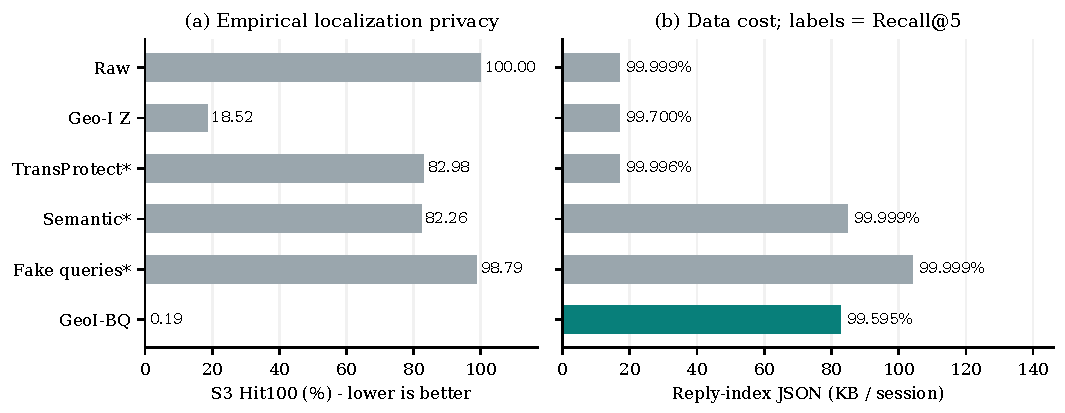
\includegraphics[width=\linewidth]{figures/tradeoff.pdf}
\captionof{figure}{So sánh trên cùng cohort. Trái: S3 Hit100 thấp hơn có lợi cho privacy. Phải: reply-index JSON KB/phiên;
nhãn là session Recall@5. Đồ thị thể hiện ba mặt của đánh đổi, không gộp thành một score tùy ý. Dấu * chỉ adaptation.}
\label{fig:tradeoff}
\end{center}
\par\smallskip\noindent\begin{tabularx}{\linewidth}{@{}P{3.6cm}XXXXX@{}}\toprule
\textbf{Phương pháp} & \textbf{Packet} & \textbf{Query điểm} & \textbf{Request KB} & \textbf{Reply KB} & \textbf{Sinh / tick ms} \\
\midrule
Raw GPS & 31{,}00 & 31{,}00 & 5{,}846 & 16{,}843 & <0{,}001 \\
Geo-I/REM Z (K1) & 31{,}00 & 31{,}00 & 6{,}352 & 16{,}921 & -- \\
TransProtect* & 31{,}00 & 31{,}00 & 6{,}351 & 16{,}847 & 3{,}287 \\
Semantic correlation* & 31{,}00 & 155{,}00 & 31{,}754 & 84{,}770 & 0{,}993 \\
Fake-query insertion* & 38{,}04 & 190{,}21 & 39{,}418 & 104{,}033 & 0{,}759 \\
\textbf{GeoI-BQ v1} & 31{,}00 & 155{,}00 & 31{,}756 & 82{,}557 & -- \\
\bottomrule\end{tabularx}\par\smallskip

Trung bình mỗi phiên 600 s; KB = 1.000 byte. ``Query điểm'' đếm từng tọa độ, gồm mọi category theo cùng
provider API. Fake-query gửi trung bình 38,04 packets thay vì 31; mọi packet phụ đều được tính.
GeoI-BQ dùng 155 point queries, cùng mức K5 như Semantic* nhưng nhiều hơn singleton Z/TransProtect*.
Chi phí này giúp lấy ứng viên đủ rộng mà không gửi nhu cầu thật.

``Sinh/tick'' là tổng thời gian sinh adapter mới chia 31 input ticks; không là p95 hay latency end-to-end.
GeoI-BQ và REM-Z được replay từ outputs cũ nên không có generation timing đồng bộ trong trial này (ký hiệu --).
Service replay dùng shared warm cache và thứ tự chạy; không dùng nó để tuyên bố phương pháp nào nhanh hơn.
Byte chỉ gồm request/reply-index JSON, chưa gồm metadata POI đầy đủ, HTTP/TLS, mạng hay năng lượng thiết bị.

\clearpage
\subsubsection{Metrics gốc: giữ đúng hợp đồng}
\par\smallskip\noindent\begin{tabularx}{\linewidth}{@{}P{3.7cm}XXXXX@{}}\toprule
\textbf{Phương pháp} & \textbf{EIE S3 (m)} & \textbf{$\Delta c$ (m)} & \textbf{ASR} & \textbf{DER} & \textbf{Path count} \\
\midrule
Raw GPS & 0{,}0 & 0{,}00 & N/A & N/A & N/A \\
Geo-I/REM Z (K1) & 338{,}5 & 688{,}65 & N/A & N/A & N/A \\
TransProtect* & 54{,}4 & 47{,}44 & N/A & N/A & N/A \\
Semantic correlation* & 41{,}9 & N/A & N/A & N/A & N/A \\
Fake-query insertion* & 13{,}3 & N/A & N/A & N/A & N/A \\
\textbf{GeoI-BQ v1} & 2104{,}6 & N/A & N/A & N/A & N/A \\
\bottomrule\end{tabularx}\par\smallskip

EIE cho point estimator ở S3 chính là MAE, không tạo thêm một kết quả độc lập. Với output singleton,
Eq.13 travel-cost distortion của TransProtect được đo bằng
\[
\Delta c=\sum_{d}\pi(d)\,|c(x,d)-c(y,d)|,
\]
với tám đích/prior chọn từ TRAIN, directed shortest-path metres và quy ước disconnected của provider.
Đây là \textbf{local-target proxy}: TransProtect* khoảng 47,44 m, REM-Z khoảng 688,65 m; không phải parity
với thí nghiệm Rome/SF gốc. Q-only hoặc real+dummy không có một released singleton $y$ duy nhất,
nên Eq.13 là N/A; không lấy centroid hoặc chọn Q gần GPS thật để tạo số.

ASR cần posterior calibrated trên real-member theo định nghĩa paper; DER cần hàm similarity và threshold
tương ứng; indistinguishable-path count cần bộ kiểm tra path đúng contract nguồn. Hiện chưa đủ đầu vào
để tính các metric này một cách đối chiếu được, vì vậy giữ N/A kèm lý do thay vì đổi tên Hit100 thành ASR.

\subsection{Supporting analysis}
\textbf{Cache theo cùng provider tĩnh.} Bảng dưới dùng chính trial mới, giữ đủ sáu phương pháp.
Epoch60 tương ứng bộ nhớ từ đầu đoạn hiện tại; session tích lũy từ đầu chuyến.
\par\smallskip\noindent\begin{tabularx}{\linewidth}{@{}P{4cm}XXX@{}}\toprule
\textbf{Phương pháp} & \textbf{Current (\%)} & \textbf{Epoch60 (\%)} & \textbf{Session (\%)} \\
\midrule
Raw GPS & 99{,}999 & 99{,}999 & 99{,}999 \\
Geo-I/REM Z (K1) & 98{,}610 & 98{,}610 & 99{,}700 \\
TransProtect* & 99{,}996 & 99{,}996 & 99{,}996 \\
Semantic correlation* & 99{,}999 & 99{,}999 & 99{,}999 \\
Fake-query insertion* & 99{,}999 & 99{,}999 & 99{,}999 \\
\textbf{GeoI-BQ v1} & 96{,}780 & 97{,}123 & 99{,}595 \\
\bottomrule\end{tabularx}\par\smallskip

Cache giúp coverage tại GPS đang xét khi tập ứng viên hợp lệ lớn hơn. Nó không bảo đảm Recall tăng theo
thời gian người dùng di chuyển, và không tự suy ra metadata vẫn đúng khi giờ mở cửa/giá/trạng thái thay đổi.

\textbf{Response depth và GPS local.} Cấu hình hiện tại dùng L60 mỗi loại/Q. Reference local ở grid 20 s
đo chất lượng mà người dùng thực sự nhận được; protected GPS vẫn được pacing 60 s và cap riêng.
Không tính local ranking là một lần phát GPS mới. Thử nghiệm L30 trên cùng Q và ablation nội bộ ngày
14/10 chỉ được giữ ở Phụ lục C; chúng không đứng thay cho so sánh paper ở bảng chính.

\textbf{Tính bất biến và kiểm chứng.} Protocol/source pins được chốt trước generation đối chứng;
không thay defense sau TEST. Mỗi arm hoàn tất 120/120 TEST, không failure. Nếu có failure,
privacy thiếu coverage là N/A, utility không giao được là 0. Các tests bao phủ split không giao family, prefix không phụ thuộc
tương lai, stripping nhãn riêng khỏi feature API, cửa sổ cùng thời gian, cache causal và tính đủ fake events.
Verifier độc lập tái tính 392.832 ô utility, 600 family-level privacy scores và 528 native-cost trip values;
kiểm tra 5.456 proposed prefixes và đếm 104.168 point queries trên toàn 176 trip-draws mỗi arm.
Sửa metadata request công khai
L30 thành L60 phản ánh đúng provider thực tế của nguồn cũ; Q/time, POI masks, utility và độ dài bytes không đổi.
Chi tiết và source hashes được giữ ở Phụ lục D và artifact; kết quả cũ không bị ghi đè.

\textbf{Phạm vi kết luận.} Cùng cohort, source adapters và finite bank làm phép so sánh có thể kiểm tra;
chúng không giải quyết mọi khác biệt fidelity, không xác nhận generalization ngoài thành phố và không
thay thế formal guarantee. So sánh chính cho thấy GeoI-BQ có privacy thực nghiệm tốt trong bank đang xét,
utility rất cao nhưng thấp hơn các adaptation, và cost lớn hơn phương pháp singleton.

\clearpage
\section{Summary}
\textbf{RQ1 -- privacy.} Phương pháp nối REM, noisy reuse và cap thành cận không gian cho lịch sử đã bảo vệ;
kernel chọn đoạn có common support và cận riêng cho toàn transcript. Hậu xử lý dẫn tới cận minimum giữa
hai nhánh, cùng diễn giải posterior odds. Kết quả lý thuyết phân biệt kernel lý tưởng với mã hiện tại:
float sampler Geo-I và full upstream restore chưa được chứng nhận; fresh uniform bits và trusted ledger
vẫn là giả thiết của cận Q. Năm Q hoặc Z không công bố không tự tạo anonymity cho người/xe.

\textbf{RQ2 -- utility.} Private adaptation tăng kỳ vọng score lập kế hoạch; tăng actual utility cần proxy phù hợp.
Union/cache và ranking bảo toàn POI đã có dưới cùng GPS/request/order. Cận theo matched public-base
và cận chuyển có điều kiện không được phát biểu thành floor phổ quát. Thực nghiệm hiện tại đạt
\PrimaryRecall\% Recall với CI \PrimaryCI\%, giảm khoảng 0,4 pp so với ba adaptation gần 100\%.

\textbf{RQ3 -- đánh đổi và đối chiếu.} Trên cohort đã xem, GeoI-BQ có Hit100 thấp hơn ba adaptation trong
bank kiểm thử cho S1--S3/S9--S10. Chi phí 155 point queries/phiên cao hơn singleton controls, nhưng không
cần fake packets phụ. Benchmark được tổ chức theo output contract, bảo lưu metrics gốc khi dùng được,
N/A, failures và CIs; các kết quả không là xác nhận vượt mọi implementation chính thức của paper.

Đóng góp thực sự là đặc tả bài toán/đánh giá, thiết kế kênh Q có cận toàn phiên và phép đối chiếu tái lập,
không phải một metric MAE/Recall mới hay tuyên bố bảo vệ hoàn toàn mọi scenario.
Các bước tiếp theo gồm chứng nhận sampler/restore, phân tích nhiều phiên và side channels,
đánh giá độc lập trên thành phố/catalogue động, tái lập predictor gốc và calibration utility thực địa.
S4--S6/S8 cần mô hình target/dữ liệu bổ sung khi trở thành thực nghiệm chính. Các hướng này không
thay đổi kết luận có điều kiện và bằng chứng hiện đã được báo cáo.

\begin{small}\begin{thebibliography}{99}
\addcontentsline{toc}{section}{References}
\bibitem{transprotect} S. Yadav, C. Yu, X. Xie, Y. Huang và C. Qiu. Protecting Vehicle Location Privacy with Contextually-Driven Synthetic Location Generation. ACM SIGSPATIAL 2024. \href{https://arxiv.org/abs/2409.09495}{DOI: 10.1145/3678717.3691211}.
\bibitem{semantic} H. Liu, H. Peng và N. Zhou. A dummy-based location privacy protection scheme with semantic correlation of moving paths. Journal of King Saud University Computer and Information Sciences 38:478. \href{https://link.springer.com/article/10.1007/s44443-026-00899-w}{DOI: 10.1007/s44443-026-00899-w}.
\bibitem{fake} H. Liu, S. Hu và N. Zhou. Location privacy protection in continuous LBSs: enhancing anonymity via fake queries. Journal of King Saud University Computer and Information Sciences 38:53. \href{https://link.springer.com/article/10.1007/s44443-025-00438-z}{DOI: 10.1007/s44443-025-00438-z}.
\bibitem{ev} U. I. Atmaca, S. Biswas, C. Maple và C. Palamidessi. A privacy-preserving querying mechanism with high utility for electric vehicles. IEEE Open Journal of Vehicular Technology 5:262--277. \href{https://wrap.warwick.ac.uk/id/eprint/183198/}{DOI: 10.1109/OJVT.2024.3360302}.
\bibitem{cpcrok} J. Wang, H. Li, Y. Sun, C. Phillips, A. Mylonas và D. Gritzalis. CPCROK: A Communication-Efficient and Privacy-Preserving Scheme for Low-Density Vehicular Ad Hoc Networks. Future Internet 17(4):165. \href{https://uhra.herts.ac.uk/id/eprint/25705/}{DOI: 10.3390/fi17040165}.
\bibitem{dpfetc} B. Yue, S. Li, A. Liu và X. Li. DP-FETC: a differentially private trajectory publishing method based on feature extraction and trajectory correlation. Electronic Research Archive 33(11):6631--6651. \href{https://www.aimspress.com/article/doi/10.3934/era.2025293}{DOI: 10.3934/era.2025293}.
\bibitem{ptppm} M. Min và cộng sự. Road Network-Aware Personalized Trajectory Protection with Differential Privacy under Spatiotemporal Correlations. arXiv:2511.21020, preprint. \href{https://arxiv.org/abs/2511.21020}{DOI: 10.48550/arXiv.2511.21020}.
\bibitem{sok} E. Buchholz, A. Abuadbba, S. Wang, S. Nepal và S. S. Kanhere. SoK: Can Trajectory Generation Combine Privacy and Utility?. Proceedings on Privacy Enhancing Technologies 2024(3):75--93. \href{https://petsymposium.org/popets/2024/popets-2024-0068.pdf}{DOI: 10.56553/popets-2024-0068}.
\bibitem{geoi} M. E. Andrés, N. E. Bordenabe, K. Chatzikokolakis và C. Palamidessi. Geo-Indistinguishability: Differential Privacy for Location-Based Systems. ACM CCS 2013, pp.901--914. \href{https://arxiv.org/abs/1212.1984}{Nguồn tác giả}.
\bibitem{predictive} K. Chatzikokolakis, C. Palamidessi và M. Stronati. A Predictive Differentially-Private Mechanism for Mobility Traces. Privacy Enhancing Technologies 2014. \href{https://petsymposium.org/2014/papers/Chatzikokolakis.pdf}{Nguồn tác giả}.

\end{thebibliography}\end{small}
\clearpage
\section*{Phụ lục A. Khoảng tin cậy privacy đầy đủ}
\addcontentsline{toc}{section}{Phụ lục A. Khoảng tin cậy privacy đầy đủ}
Mỗi hàng là một method/task; CI95\% percentile bootstrap 10.000 lần theo family.
MAE và Hit được chọn attacker riêng theo loss trên SELECTION. Mẫu số TEST là 20 family, 120 trip-draw/arm;
S1/S3 trung bình 31 targets/trip, các task còn lại một target/trip. Dấu * là adaptation.
CI [0;0] khi không thấy hit trong mẫu chỉ là kết quả bootstrap thực nghiệm, không là chứng nhận rủi ro bằng 0.
\begin{footnotesize}\par\smallskip\noindent\begin{tabularx}{\linewidth}{@{}P{3.4cm}P{.7cm}XXXX@{}}\toprule
\textbf{Phương pháp} & \textbf{Case} & \textbf{Hit100\%} & \textbf{CI95\% Hit} & \textbf{MAE m} & \textbf{CI95\% MAE} \\
\midrule
Raw GPS & S1 & 100{,}000 & [100{,}000; 100{,}000] & 0{,}0 & [0{,}0; 0{,}0] \\
Raw GPS & S2 & 100{,}000 & [100{,}000; 100{,}000] & 0{,}0 & [0{,}0; 0{,}0] \\
Raw GPS & S3 & 100{,}000 & [100{,}000; 100{,}000] & 0{,}0 & [0{,}0; 0{,}0] \\
Raw GPS & S9 & 100{,}000 & [100{,}000; 100{,}000] & 0{,}0 & [0{,}0; 0{,}0] \\
Raw GPS & S10 & 100{,}000 & [100{,}000; 100{,}000] & 0{,}0 & [0{,}0; 0{,}0] \\
Geo-I/REM Z (K1) & S1 & 18{,}522 & [14{,}892; 22{,}204] & 338{,}5 & [319{,}0; 359{,}8] \\
Geo-I/REM Z (K1) & S2 & 37{,}500 & [29{,}167; 45{,}833] & 214{,}3 & [171{,}2; 261{,}2] \\
Geo-I/REM Z (K1) & S3 & 18{,}522 & [14{,}892; 22{,}204] & 338{,}5 & [319{,}0; 359{,}8] \\
Geo-I/REM Z (K1) & S9 & 5{,}833 & [2{,}500; 10{,}000] & 435{,}8 & [380{,}2; 498{,}0] \\
Geo-I/REM Z (K1) & S10 & 35{,}000 & [26{,}667; 43{,}333] & 246{,}8 & [201{,}5; 297{,}8] \\
TransProtect* & S1 & 82{,}984 & [79{,}973; 85{,}672] & 54{,}4 & [47{,}9; 62{,}0] \\
TransProtect* & S2 & 94{,}167 & [88{,}333; 98{,}333] & 28{,}7 & [20{,}4; 39{,}1] \\
TransProtect* & S3 & 82{,}984 & [79{,}973; 85{,}672] & 54{,}4 & [47{,}9; 62{,}0] \\
TransProtect* & S9 & 96{,}667 & [92{,}500; 100{,}000] & 17{,}8 & [8{,}5; 29{,}3] \\
TransProtect* & S10 & 90{,}833 & [84{,}167; 96{,}667] & 33{,}6 & [23{,}2; 46{,}6] \\
Semantic correlation* & S1 & 82{,}258 & [77{,}097; 86{,}532] & 41{,}9 & [38{,}1; 46{,}1] \\
Semantic correlation* & S2 & 100{,}000 & [100{,}000; 100{,}000] & 8{,}2 & [5{,}1; 13{,}0] \\
Semantic correlation* & S3 & 82{,}258 & [77{,}097; 86{,}532] & 41{,}9 & [38{,}1; 46{,}1] \\
Semantic correlation* & S9 & 100{,}000 & [100{,}000; 100{,}000] & 5{,}3 & [5{,}0; 5{,}8] \\
Semantic correlation* & S10 & 100{,}000 & [100{,}000; 100{,}000] & 7{,}3 & [5{,}4; 10{,}6] \\
Fake-query insertion* & S1 & 53{,}387 & [41{,}156; 65{,}215] & 1213{,}0 & [907{,}7; 1539{,}9] \\
Fake-query insertion* & S2 & 92{,}500 & [85{,}000; 99{,}167] & 239{,}1 & [44{,}8; 481{,}7] \\
Fake-query insertion* & S3 & 98{,}790 & [97{,}957; 99{,}462] & 13{,}3 & [9{,}8; 18{,}5] \\
Fake-query insertion* & S9 & 99{,}167 & [97{,}500; 100{,}000] & 42{,}2 & [4{,}8; 116{,}4] \\
Fake-query insertion* & S10 & 100{,}000 & [100{,}000; 100{,}000] & 6{,}4 & [5{,}2; 7{,}9] \\
\textbf{GeoI-BQ v1} & S1 & 0{,}188 & [0{,}000; 0{,}565] & 2104{,}6 & [1784{,}5; 2436{,}0] \\
\textbf{GeoI-BQ v1} & S2 & 0{,}000 & [0{,}000; 0{,}000] & 2124{,}2 & [1789{,}4; 2462{,}4] \\
\textbf{GeoI-BQ v1} & S3 & 0{,}188 & [0{,}000; 0{,}565] & 2104{,}6 & [1784{,}5; 2436{,}0] \\
\textbf{GeoI-BQ v1} & S9 & 0{,}000 & [0{,}000; 0{,}000] & 1986{,}4 & [1626{,}2; 2343{,}0] \\
\textbf{GeoI-BQ v1} & S10 & 0{,}000 & [0{,}000; 0{,}000] & 2124{,}2 & [1789{,}4; 2462{,}4] \\
\bottomrule\end{tabularx}\par\smallskip
\end{footnotesize}

\clearpage
\section*{Phụ lục B. Chênh lệch utility theo purpose}
\addcontentsline{toc}{section}{Phụ lục B. Chênh lệch utility theo purpose}
Đơn vị điểm phần trăm: GeoI-BQ trừ đối chứng, cùng session cache. Tất cả controls/purposes được giữ,
không chỉ các chênh lệch có lợi. Bootstrap ghép family dùng cùng draw/trip workload.
\begin{small}\par\smallskip\noindent\begin{tabularx}{\linewidth}{@{}P{3.5cm}P{2.4cm}XX@{}}\toprule
\textbf{Đối chứng} & \textbf{Purpose} & \textbf{BQ trừ control (pp)} & \textbf{CI95\% (pp)} \\
\midrule
Raw GPS & Trung bình & -0{,}404 & [-0{,}775; -0{,}095] \\
Raw GPS & Gần nhất & -0{,}362 & [-0{,}720; -0{,}070] \\
Raw GPS & Nhanh nhất & -0{,}359 & [-0{,}715; -0{,}070] \\
Raw GPS & Bán kính & -0{,}612 & [-1{,}324; -0{,}106] \\
Raw GPS & Ít vòng đường & -0{,}282 & [-0{,}634; -0{,}047] \\
Geo-I/REM Z (K1) & Trung bình & -0{,}105 & [-0{,}542; 0{,}275] \\
Geo-I/REM Z (K1) & Gần nhất & -0{,}114 & [-0{,}524; 0{,}241] \\
Geo-I/REM Z (K1) & Nhanh nhất & -0{,}112 & [-0{,}519; 0{,}242] \\
Geo-I/REM Z (K1) & Bán kính & -0{,}237 & [-1{,}006; 0{,}338] \\
Geo-I/REM Z (K1) & Ít vòng đường & 0{,}044 & [-0{,}381; 0{,}389] \\
TransProtect* & Trung bình & -0{,}401 & [-0{,}773; -0{,}093] \\
TransProtect* & Gần nhất & -0{,}362 & [-0{,}720; -0{,}070] \\
TransProtect* & Nhanh nhất & -0{,}359 & [-0{,}715; -0{,}070] \\
TransProtect* & Bán kính & -0{,}612 & [-1{,}324; -0{,}106] \\
TransProtect* & Ít vòng đường & -0{,}273 & [-0{,}622; -0{,}040] \\
Semantic correlation* & Trung bình & -0{,}404 & [-0{,}775; -0{,}096] \\
Semantic correlation* & Gần nhất & -0{,}362 & [-0{,}720; -0{,}070] \\
Semantic correlation* & Nhanh nhất & -0{,}359 & [-0{,}715; -0{,}070] \\
Semantic correlation* & Bán kính & -0{,}612 & [-1{,}324; -0{,}106] \\
Semantic correlation* & Ít vòng đường & -0{,}285 & [-0{,}637; -0{,}050] \\
Fake-query insertion* & Trung bình & -0{,}404 & [-0{,}775; -0{,}096] \\
Fake-query insertion* & Gần nhất & -0{,}362 & [-0{,}720; -0{,}070] \\
Fake-query insertion* & Nhanh nhất & -0{,}359 & [-0{,}715; -0{,}070] \\
Fake-query insertion* & Bán kính & -0{,}612 & [-1{,}324; -0{,}106] \\
Fake-query insertion* & Ít vòng đường & -0{,}285 & [-0{,}635; -0{,}051] \\
\bottomrule\end{tabularx}\par\smallskip
\end{small}
CI tuyệt đối từng purpose và chênh lệch so với TransProtect*:
\begin{small}\par\smallskip\noindent\begin{tabularx}{\linewidth}{@{}P{3.2cm}XXX@{}}\toprule
\textbf{Purpose} & \textbf{BQ Recall (\%)} & \textbf{CI95\% tuyệt đối} & \textbf{Δ so TransProtect* (pp), CI95\%} \\
\midrule
Trung bình & 99{,}595 & [99{,}224; 99{,}903] & -0{,}401; [-0{,}773; -0{,}093] \\
Gần nhất & 99{,}638 & [99{,}280; 99{,}930] & -0{,}362; [-0{,}720; -0{,}070] \\
Nhanh nhất & 99{,}641 & [99{,}285; 99{,}930] & -0{,}359; [-0{,}715; -0{,}070] \\
Bán kính & 99{,}388 & [98{,}676; 99{,}894] & -0{,}612; [-1{,}324; -0{,}106] \\
Ít vòng đường & 99{,}712 & [99{,}362; 99{,}946] & -0{,}273; [-0{,}622; -0{,}040] \\
\bottomrule\end{tabularx}\par\smallskip
\end{small}

\clearpage
\section*{Phụ lục C. Bằng chứng giải thích nội bộ, tách khỏi trial mới}
\addcontentsline{toc}{section}{Phụ lục C. Bằng chứng giải thích nội bộ, tách khỏi trial mới}
Các bảng này thuộc \texttt{main\_depth\_20261014\_v1}, không phải các phương pháp từ paper.
Mục đích là giải thích thiết kế và response depth; không ghép privacy scores/CI lịch sử thành phép
so sánh trực tiếp với ba adaptation ở Phần 4. GeoI-BQ được phát lại từ nguồn này nên utility khớp đúng.
\par\smallskip\noindent\begin{tabularx}{\linewidth}{@{}P{4cm}XXXXX@{}}\toprule
\textbf{Ablation14/10} & \textbf{Trung bình} & \textbf{Gần nhất} & \textbf{Nhanh nhất} & \textbf{Bán kính} & \textbf{Ít vòng đường} \\
\midrule
Service-cover K5 & 100{,}000 & 100{,}000 & 100{,}000 & 100{,}000 & 100{,}000 \\
Initial-only & 98{,}377 & 98{,}984 & 98{,}987 & 96{,}358 & 99{,}181 \\
Local explore & 99{,}562 & 99{,}609 & 99{,}609 & 99{,}358 & 99{,}670 \\
Public-base $\Gamma=0$ & 99{,}711 & 99{,}730 & 99{,}731 & 99{,}642 & 99{,}740 \\
GeoI-BQ v1 & 99{,}595 & 99{,}638 & 99{,}641 & 99{,}388 & 99{,}712 \\
\bottomrule\end{tabularx}\par\smallskip

Public-base $\Gamma=0$ có macro 99,711\%, cao hơn 99,595\% của cấu hình chính trong trial nội bộ này.
Điều đó nhất quán với việc điểm proxy không bảo đảm actual Recall luôn tăng; không đổi mô hình chính
sau khi thấy chênh lệch. Service-cover gần 100\% là một control nội bộ, không là SOTA từ paper.

\textbf{L30 so với L60 trên cùng Q/time.} Đây là truncation phản hồi, không lấy mẫu lại Q hay chọn chuyến.
\par\smallskip\noindent\begin{tabularx}{\linewidth}{@{}P{3cm}XXX@{}}\toprule
\textbf{Purpose} & \textbf{L30 cùng Q (\%)} & \textbf{L60 trừ L30 (pp)} & \textbf{CI95\% (pp)} \\
\midrule
Trung bình & 94{,}170 & 5{,}425 & [3{,}486; 7{,}527] \\
Gần nhất & 96{,}105 & 3{,}534 & [2{,}371; 4{,}726] \\
Nhanh nhất & 96{,}101 & 3{,}540 & [2{,}375; 4{,}740] \\
Bán kính & 89{,}015 & 10{,}374 & [5{,}768; 15{,}706] \\
Ít vòng đường & 95{,}459 & 4{,}253 & [2{,}946; 5{,}520] \\
\bottomrule\end{tabularx}\par\smallskip

Giữ L60 vì workload hiện tại cho coverage tốt hơn; không khẳng định 60 tối ưu cho mọi catalogue.
App trả danh sách phù hợp đã sắp xếp; Recall@5 là phép đo, không là output contract top-five.

\clearpage
\section*{Phụ lục D. Tái lập, fidelity và nguồn số liệu}
\addcontentsline{toc}{section}{Phụ lục D. Tái lập, fidelity và nguồn số liệu}
\textbf{Artifact chính:} \texttt{artifacts/benchmarks/paper\_comparison\_20261028\_v1/}.
Protocol chốt nguồn và cấu hình trước generation; source snapshot, families, predictions, models,
selection logs, native metrics, failures và bảng kết quả được lưu cùng phiên bản. Khoá randomness riêng
không nằm trong repository; outputs công khai đủ để replay evaluation mà không công bố seed cho attacker.

\textbf{Quy trình kiểm tra:}
\begin{enumerate}
\item Cài môi trường theo \texttt{requirements-paper-comparison.txt}; giữ phiên bản và thread environment trong protocol.
\item Từ repo root, chạy \texttt{python -m} với module
\texttt{experiments.check\_paper\_comparison\_20261028} để replay verifier ở chế độ chỉ đọc.
Không gọi lại generation hoặc ghi đè receipt đã đóng băng.
\item Trong thư mục report, chạy \texttt{python build\_report.py --check}; bảng chính đọc duy nhất trial mới,
bảng phụ đọc nguồn 14/10 được đánh dấu riêng.
\item Dựng bằng \texttt{tectonic --keep-logs report\_explained.tex}, render từng trang.
Sau khi xem render, chạy validator với cờ \texttt{--visual-reviewed}.
\end{enumerate}

\textbf{Fidelity mappings:} \texttt{docs/reproduction/transprotect.md},
\texttt{semantic\_correlation.md} và \texttt{fake\_queries.md} ghi công thức/cơ chế giữ lại và phần thay thế.
Markov không được gọi là Transformer; public POI semantics không được gọi là AMap semantic ground truth.
Không sử dụng benchmark của AnotherMe offline để điền ô online còn thiếu.

\textbf{Sai khác metadata đã xử lý:} nguồn 14/10 có trường request \texttt{response\_l=30}, trong khi callback
provider luôn trả top60 và không đọc trường này. Trial mới chuẩn hóa trường đó thành 60 cho mọi arm.
Verifier kiểm tra exact Q/time, reply masks, utility và byte counts; 30/60 có cùng độ dài JSON.
Đây là sửa hợp đồng công khai khi replay, không thay defense hay ghi đè artifact cũ.

\textbf{Bảng nối chứng minh--mã.}

\begin{footnotesize}
\begin{tabularx}{\linewidth}{@{}P{2.6cm}P{4cm}Y@{}}\toprule
\textbf{Kết quả} & \textbf{Giả thiết / cơ chế trong mã} & \textbf{Kiểm chứng và phạm vi}\\\midrule
Mệnh đề 1--2 & \texttt{RoadExponential}, \texttt{PrivateReuseSMREM}; prospective cap & Tam giác/Lipschitz, oracle cost 0/1/2; sampler float và full restore chưa được chứng nhận.\\
Mệnh đề 3 & \texttt{FiniteCenteredKernel}; common library/base; bounded score & Exact normalization/PMF/ratio bằng số hữu tỷ; cần bit đều mới.\\
Mệnh đề 4 & \texttt{BoundedQuerySession}; ledger, commit ba khung & Prefix budget, restart/retry, support/đường và hidden-lane oracle; không reset phiên.\\
Toàn transcript/Bayes & \texttt{finite\_session\_bounds}; cùng provider law và clock & Hợp thành, chiếu augmented history xuống wire; identity/future chỉ có hệ quả có điều kiện.\\
Utility gain/path & \texttt{conditional\_gain}, whole-path $\chi^2$ & Gain score và cận matched-base; actual gain cần covariance/calibration.\\
Cache/transfer & \texttt{local\_sorted\_pois}, \texttt{reference\_transfer} & Replies hợp lệ, cùng GPS/order; sai số TV/proxy chưa biết không được đặt bằng 0.\\\bottomrule
\end{tabularx}
\end{footnotesize}
Các oracle không chứng nhận continuous float sampler hay full upstream restoration. Bảng điều kiện cuối
Phần~\ref{sec:utilityproof} phải được đọc cùng định lý, không tách kết luận khỏi giả thiết.
\texttt{report\_sources.json} giữ hashes đầu vào; \texttt{report\_manifest.json} ghi kiểm tra bảng/PDF
và phạm vi visual QA. \texttt{literature\_evidence.json} giữ metadata, coverage và link nguồn từng paper.

\end{document}
